\documentclass{article}
\usepackage[english]{babel}

\usepackage[a4paper,top=2cm,bottom=2cm,left=3cm,right=3cm,marginparwidth=1.75cm]{geometry}
\usepackage{amsmath}
\usepackage{graphicx}
\usepackage[colorlinks=true, allcolors=blue]{hyperref}
\usepackage{listings}
\usepackage{minted}
\setlength{\parindent}{0pt}

\title{Physics of Complex Systems: Exercise 1}
\author{Leopold Schaller and Daniel Lender}

\begin{document}
\maketitle

\section*{Task 1.1: Random numbers}
\subsection*{(a)}
We generate pseudo random numbers in python using the implemented PCG64 (Permutated Congruential Generator).
\vspace{-8pt}
\begin{minted}{Python}
rng   = np.random.default_rng()
rints = rng.integers(low=0, high=10, size=10000)
\end{minted}

\subsection*{(b)}
We count the frequency of the generated numbers:
\vspace{-8pt}
\begin{minted}{Python}
count = {}                                           
for n in rints:
    count[n] = count.get(n,0)+1
\end{minted}

And create a bar chart (technically no real histogram, but it has a better visibility):
\vspace{-8pt}
\begin{minted}{Python}
c = [count[n] for n in range(10)]
x = np.arange(10)
plt.bar(x, c, color='skyblue')
\end{minted}
\begin{figure}[h!]
    \centering
    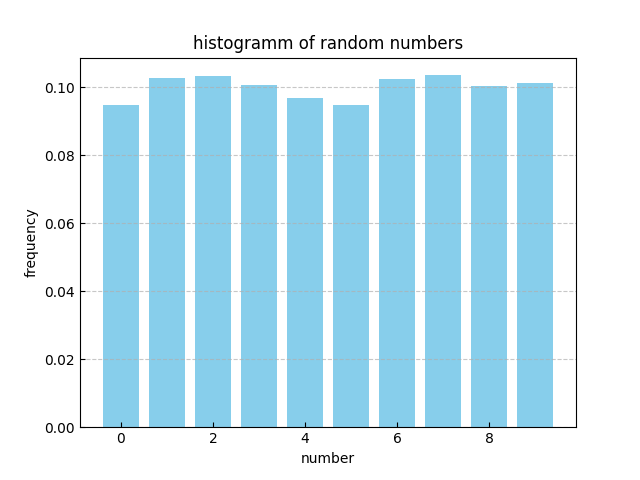
\includegraphics[width=0.5\linewidth]{histogram.png}
    \caption{Histogram of 10.000 generated random numbers}
\end{figure}

\subsection*{(c)}
We'd expect a standard deviation of a binomial distribution $\sigma=\sqrt{N\cdot p\cdot (1-p)}=30$, i.e., We expect 68\% of the time the count will be $1000\pm30$, 95\% of the time $1000\pm60$.

\subsection*{(d)}
We generate random numbers in the range [0, 9].
If we sum up two of them the number of ways z to achieve a result $x\in[0,18]$ is determined by $z(x)= 10-|9-x|$:
Therefore the total number of combinations is $z_{tot}=10^2=100$. 
Since each individual number has an equal probability of being selected (0.1), the shape of the resulting histogram is determined solely by the number of possible combinations for each sum. For two variables, this results in a linear increase toward the mean and a linear decrease toward the maximum, forming a \textbf{triangular distribution}.

In general on would write $x\in[0, K\cdot n]$, $z(x)=n-|(n-1)-x|$ and $n_{tot}=n^K$, with n, the number of different generated random numbers and K the number of random numbers summed up.\\

In the modified code, two numbers are summed up, the results are plotted as in (b).
\vspace{-8pt}
\begin{minted}{python}
K=2
rints2 = rints.reshape(-1, K).sum(axis=1)
count2 ={}             
for n in rints2:
    count2[n] = count2.get(n,0)+1 
c2 =[count2.get(n, 0) for n in range(9*K+1)]
x2 = np.arange(9*K+1)
plt.bar(x2, c2, color='firebrick')
\end{minted}
reshape(-1, K) folds a list of integers (here rints) into a matrix with K columns, -1 tells the computer to calculate the amount of rows needed. 
sum(axis=1) sums all columns, sum(axis=0) would sum all rows.

\begin{figure}[h]
    \centering
    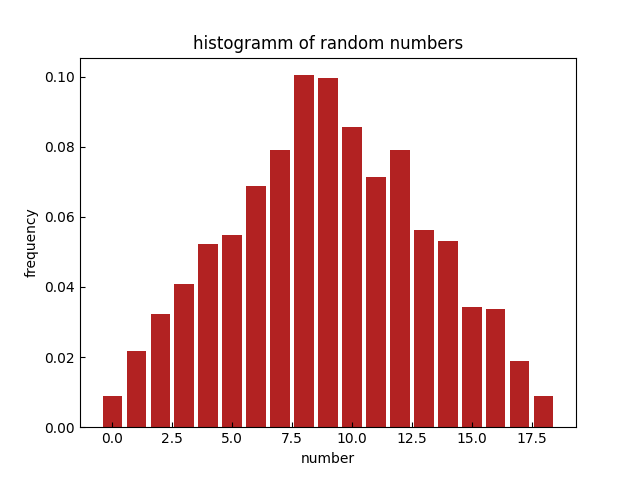
\includegraphics[width=0.8\linewidth]{histogram_k2.png}
    \caption{Histogram
    for K=2 and 10.000 generated random numbers}
\end{figure}
\subsection*{(e)}
For large K values the distribution approximates a normal/Gaussian distribution, where the expectation value for the sume is $S = K * 4.5$. Therefore the code was changed to generate columns with 20 numbers and the amount of generated numbers is $N = 1000000$.
\begin{figure}[h!]
    \centering
    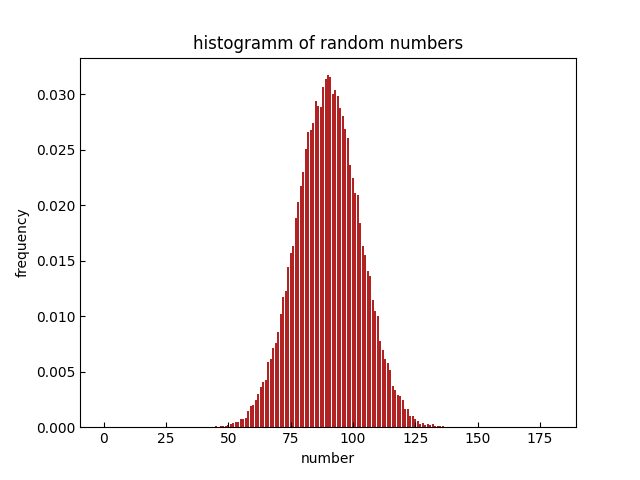
\includegraphics[width=0.8\linewidth]{histogram_k20.png}
    \caption{Histogram for K=20 and one million generated random numbers}
\end{figure}

\end{document}

# In Pycharm, you have to do this in the Terminal:
# latexmk -pdf -shell-escape exercise1_Schaller_Lender.tex